\documentclass[12pt]{article}

\usepackage{latex/ediArticle}  %from ediArticle.sty
%\usepackage{multirow}
\usepackage{amsmath}
%\usepackage{amssymb}
%\usepackage[normalem]{ulem}
%\usepackage[table]{xcolor}
\usepackage{lineno}
\linenumbers

%%%%%%%%%%%%%%%%%%%%%%%%%%%%%%%%%%%%%%%%%%%%%%%%%%%%%%
\title{\LARGE \bfseries \vspace{-2cm} Burden and health-related quality of life among caregivers of people with motor neuron disease}
\author{\vspace{-2cm}}
\date{\vspace{-2cm}}

\begin{document}

% Set font size to 13pt
\fontsize{13pt}{15pt}\selectfont

\maketitle


%%%%%%%%%%%%%%%%%%%%%%%%%%%%%%%%%%%%%%%%%%%%%%%%%%%%%%
\section*{Introduction}
Motor neuron disease (MND) is a progressive neurodegenerative disease that impacts not only patients but also their informal caregivers. Several studies on ALS in Australia \parencite{lillo_caregiver_2012}, United States \parencite{qutub_life_2014, burke_caregiver_2015, roach_dynamics_2009}, Turkey \parencite{tulek_care_2023}, Ireland \parencite{galvin_caregiving_2016}, Germany \parencite{schischlevskij_informal_2021}, and China \parencite{geng_patients_2017}, have investigated the factors contributing to caregiver burden in ALS and the associated impact of caregiving on the quality of life of these individuals. \textcite{lillo_caregiver_2012} found that patients' abnormal behavior and caregiver stress were the strongest predictors of high caregiver burden, while physical disability was not significantly associated. 

A cross-sectional study of 33 patient-caregiver pairs, which showed that high caregiver burden was associated with greater patient apathy, disinhibition, and executive dysfunction, as well as caregiver distress \parencite{burke_caregiver_2015}. \textcite{qutub_life_2014} study also found that patients' functional status did not affect caregivers' burden. \textcite{schischlevskij_informal_2021} results showed that caregiver burden increased with patients' decline in functional status - patients' wheelchair use and need for supervision were the strongest predictors of burden.

\textcite{tulek_care_2023} study corroborates sex as having a significant relationship to caregivers' burden. \textcite{geng_patients_2017} found an association between caregiver burden and older caregiver age. Other factors related to caregivers' burden are difficulties in managing ALS, the emotional or psychosocial impact of caregiving, limitations or restrictions, and the effects on relationships that caregiving has on the caregivers \parencite{galvin_caregiving_2016}. Patients' functional status affect caregiver quality of life \parencite{roach_dynamics_2009}.

%%%%%%%%%%%%%%%%%%%%%%%%%%%%%%%%%%%%%%%%%%%%%%%%%%%%%%
\section*{Methods}

\subsection*{Study design and participants}
COMMEND was a XXX designed to YYY. The study design, patient
characteristics, and baseline costs and resource-use data
have been reported \parencite{gould_randomised_2022}. The present study focuses on the caregivers; the baseline characteristics and quality of life have been reported previously for patient  \parencite{gould_acceptance_2024}. Patients with
probable/confirmed?? MND, CRITERIA???, were enrolled between
DATE and DATE, mostly at WHERE. Patients were
also required??? to have a primary caregiver who was
willing to participate in the study. Caregivers were included if BRIEF INCLUSION CRITERIA [cite trial]. 

\subsection*{Data and questionnaires}
Data were collected for patients and caregivers at the
baseline visit and at baseline, 6 months, and 18 months during WHICH?? visits. Full details of the baseline patient and caregiver
demographics and characteristics, including comorbidities
and medications used, have been reported previously \parencite{gould_acceptance_2024, keetharuth_costeffectiveness_2024}.

% Paraphrase this
We assessed caregiver burden at every visit using the 22-item version of Zarit Burden Interview (ZBI). ZBI is a widely-used instrument for assessing the perceived burden experienced by caregivers \parencite{zarit_relatives_1980}. The questions cover the caregiver’s health, psychological well-being, finances, social life, and relationship with the patient. The 22-item version of ZBI contains five-point Likert-style questions with responses to each item ranging from 0, denoting “never”, to 4, denoting “nearly always”. \parencite{zarit_hidden_1985}. The total score therefore ranges from 0 to 88, with a higher score indicating a greater perceived care burden. 

% Paraphrase this and shorten
Caregivers self-assessed their HRQoL at using the EuroQol Visual Analogue Scale (EQ-VAS) and 5-dimension (EQ-5D) questionnaires [\textbf{REF}]. For EQ-5D, they scored their current health state in each of five domains (pain/discomfort, anxiety/depression, mobility, usual activities, and self-care) using a 3-point scale (no, moderate, or extreme problems). From the health-state profile obtained, a scoring algorithm using English preference weights [\textbf{REF}] was used to calculate a total utility score (EQ-5D index score) between 0 (represents death) and 1.0 (represents perfect health). Caregivers rated their current health status on the day of assessment using EQ-VAS, which ranges from 0 (worst imaginable health) to 100 (best possible health). The mean norm value in the English population is reportedly XX (\textbf{REF}). 

Factors related to the informal caregivers (\autoref{tab_var_category}), that is age,sex, educational level, work status, change in work status, relation to the patient with ALS, and whether cohabiting with the patient, was collected with the study‐specific questionnaire. It also included questions on time spent on informal caregiving in personal ADL (P‐ADL),that is feeding, bathing, dressing, toileting and transfer; instrumental ADL (I‐ADL), that is cooking, transport, cleaning and shopping; andother activities that the patient with ALS used to do before disease onset. The first set of variables were caregiver sociodemographic characteristics.  such as sex (DEFINE), age (DEFINE), level of education (DEFINE), employment status (DEFINE). We also asked respondents if they had any medical conditions. Other variables were caregiving context, including relationship with care recipient (DEFINE), intensity of caregiving activities (DEFINE), and how long has been looking after (DEFINE).

We also collected information on characteristics of patients with ALS (\autoref{tab_var_category}). These included age, sex, marital status, employment situation, educational level, presence and number of comorbidities, duration of disease, disease severity. These were collected during XXX \parencite{gould_acceptance_2024}. Disease severity was measured using the ALS Functioning Rating Scale‐Revised, ALSFRS‐R \parencite{cedarbaum_alsfrs-r_1999}. We used the algorithm developed by \textcite{balendra_estimating_2014} to calculate King's clinical stages from ALSFRS-R scores. The King's staging system is based on disease burden and consists of five disease stages (1 to 5) with stage 1 being onset of disease in one anatomical region and stage 5 being death.

\begin{table}[H]
    \centering \singlespacing \small
    \caption{Categorization of independent variables}
    \begin{tabular}{|L{6cm}|L{9cm}|}
        \hline
        \PlainInput{tables/tab_var_category}
    \end{tabular}
    \label{tab_var_category}
    \caption*{\footnotesize \textit{Notes:} Donec sit amet viverra justo}
\end{table}

\subsection*{Statistical analysis}
We described the characteristics of the participants (patients with MND and caregivers) using means and standard deviations for continuous variables and using numbers and percentages for categorical variables. We used univariate linear regression to examine the direction and size of the relationships between caregiver burden and possible influencing factors on  caregivers’ burden (ZBI) and health-related quality of life (EQ-5D). We then conducted a multiple regression analysis to test the extent to which these variables explained ZBI and EQ-5D. We selected variables to add to multiple linear regression by adopting a critical level of significance (p $\leq$ 0.10) in the univariate analysis.
%Spearman correlation coefficients examined the within- subject associations between continuous variables such as caregiver ZBI total scores, EQ-5D index scores, EQ-5D VAS scores, and T-IADL, at baseline, at 18 months, and for the change from baseline to 18 months. We inter- preted correlation coefficients of 0–0.19 as very weak and 0.20–0.39 as weak.
All analysis were conducted using Stata version 18.0 (StataCorp, College Station, Texas, USA).

\section*{Results}
At baseline, the study cohort analyzed comprised 93 caregivers that consent was obtained to participate in the study, alongside the patients in their care. Both ZBI and HRQoL data at was collected from a total of 86 caregivers at baseline, of which 85 had complete and data on all outcome measures. One caregiver-patient pair was were excluded from further analyses because the EQ-5D score was negative while the VAS score was 100, resulting in 84 full observations. %This represents about 1.5\% of an estimated 5700 patients (prevalence, 8.6 per 100,000 persons) that lived with MND in 2020 \textbf{10.1080/21678421.2019.1587629}. The total number of caregivers with available data at the 9-month timepoint (and for the change from baseline to 9 months was) was: ZBI, n = 66; EQ-5D, n = 67.

\subsection*{Caregiver and patient characteristics}
\autoref{tab_desc_stat} summarizes the baseline sociodemographic and clinical characteristics of the caregivers and patients. Caregivers had a mean (SD) age of 59.7 (11.8) years and most (70.2\%) caregivers were female, consistent with previous literature \parencite{schischlevskij_informal_2021}. Approximately half of the caregivers (4.8\%) reported being in paid employment.  Most caregivers (92.9\%) were direct family members of the patients and likely living together with a partner with MND as observed in previous studies \parencite{burke_longitudinal_2018, galvin_caregiving_2016, schischlevskij_informal_2021}. The median duration of caregiving (DOC) was three hours per day (as stated by the main CG; additional hours by more than one CG per patient are possible).  The mean ZBI scores at baseline was 21.1 (12.3). The EQ-VAS mean (79.8/100) was the same as the estimated EQ-5D-5L index score with 0.80/1. These HRQoL values were \textbf{lower/higher} than in the general British population (EQ-VAS mean = XX.X/100, SD = X.X [REF], EQ-5D-5L index value mean = X.X, SD = X.X) [REF].  

Patients had a mean (SD) age of 62.2 (10.6) years, the mean (SD) time since diagnosis was 1.6 (2.9) years, and about half had a physical or mental comorbidity (mean of 0.6 comorbidities). The mean ALSFRS-R score was 35.5/48 (a score of 48 represents an absence symptoms while 0 represents the worst functional status). The cohort included patients in all disease severity stages, but only 6\% were in King's stage 4. In summary, these characteristics mean that our cohort was relatively younger and had less severe disease compared to previous studies [REF]. 40.5\% of patients were female, consistent with literature that MND diagnosis was more common in men \parencite{burchardt_analysis_2022}.

\begin{table}[H]
    \centering \singlespacing \small
    \caption{Patients’ and caregivers characteristics, patients' functional status (ALSFRS-R), caregiver burden (ZBI score), and caregiver health-related quality of life (EQ-5D) at baseline}
    \begin{tabular}{|L{5cm}|R{3.2cm}|}
        \hline
        \PlainInput{tables/tab_desc_stat}
    \end{tabular}
    \label{tab_desc_stat}
    \caption*{\footnotesize \textit{Notes:} Data are based on participants with non-missing baseline caregiver burden and quality of life data. ALSFRS-R, Revised Amyotrophic Lateral Sclerosis Functional Rating Scale; EQ-5D, EuroQol 5-dimension questionnaire; n, number; SD, standard deviation, VAS, visual analog scale; ZBI, Zarit Burden Interview.
}
\end{table}

\subsection*{Impact of patient's functional status on caregivers}
The mean ZBI score by King's stage showed that caregivers patients with worse functional status had a greater burden, but results were not consistent. \autoref{fig:outcome-kings-stage} shows the ZBI score by King's stage at baseline, 6 months, and 9 months. The ZBI score was highest for carers of stage 4 patients, but higher for stage 2 compared to stage 3. Using baseline data only, scores were < 20 for stage 1/12 and >20 for stage 3/4. We found a weak, negative, correlation between the ZBI score and the ALSFRS-R ($\rho$ = −0.208, p < 0.002). Due to this inconsistency, functional status.

Using ANOVA on pooled data, we observed statistically significant differences in the mean EQ-5D index scores between the King’s Stages (p = 0.001, \autoref{tab_outcomes_kings}). This finding was supported by a weak, but positive, correlation between the EQ-5D index score and the ALSFRS-R ($\rho$ = 0.216, p = 0.002). Together, these imply that a better (worse) patient’s functional status is associated with led to a higher (lower) caregiver HRQoL. There was no significant association between functional status and either the mobility or self-care, suggesting that these EQ-5D domains were less useful. Similar non-significant results were observed for EQ-VAS scores (p = 0.999)

\begin{figure}[H]
    \centering
    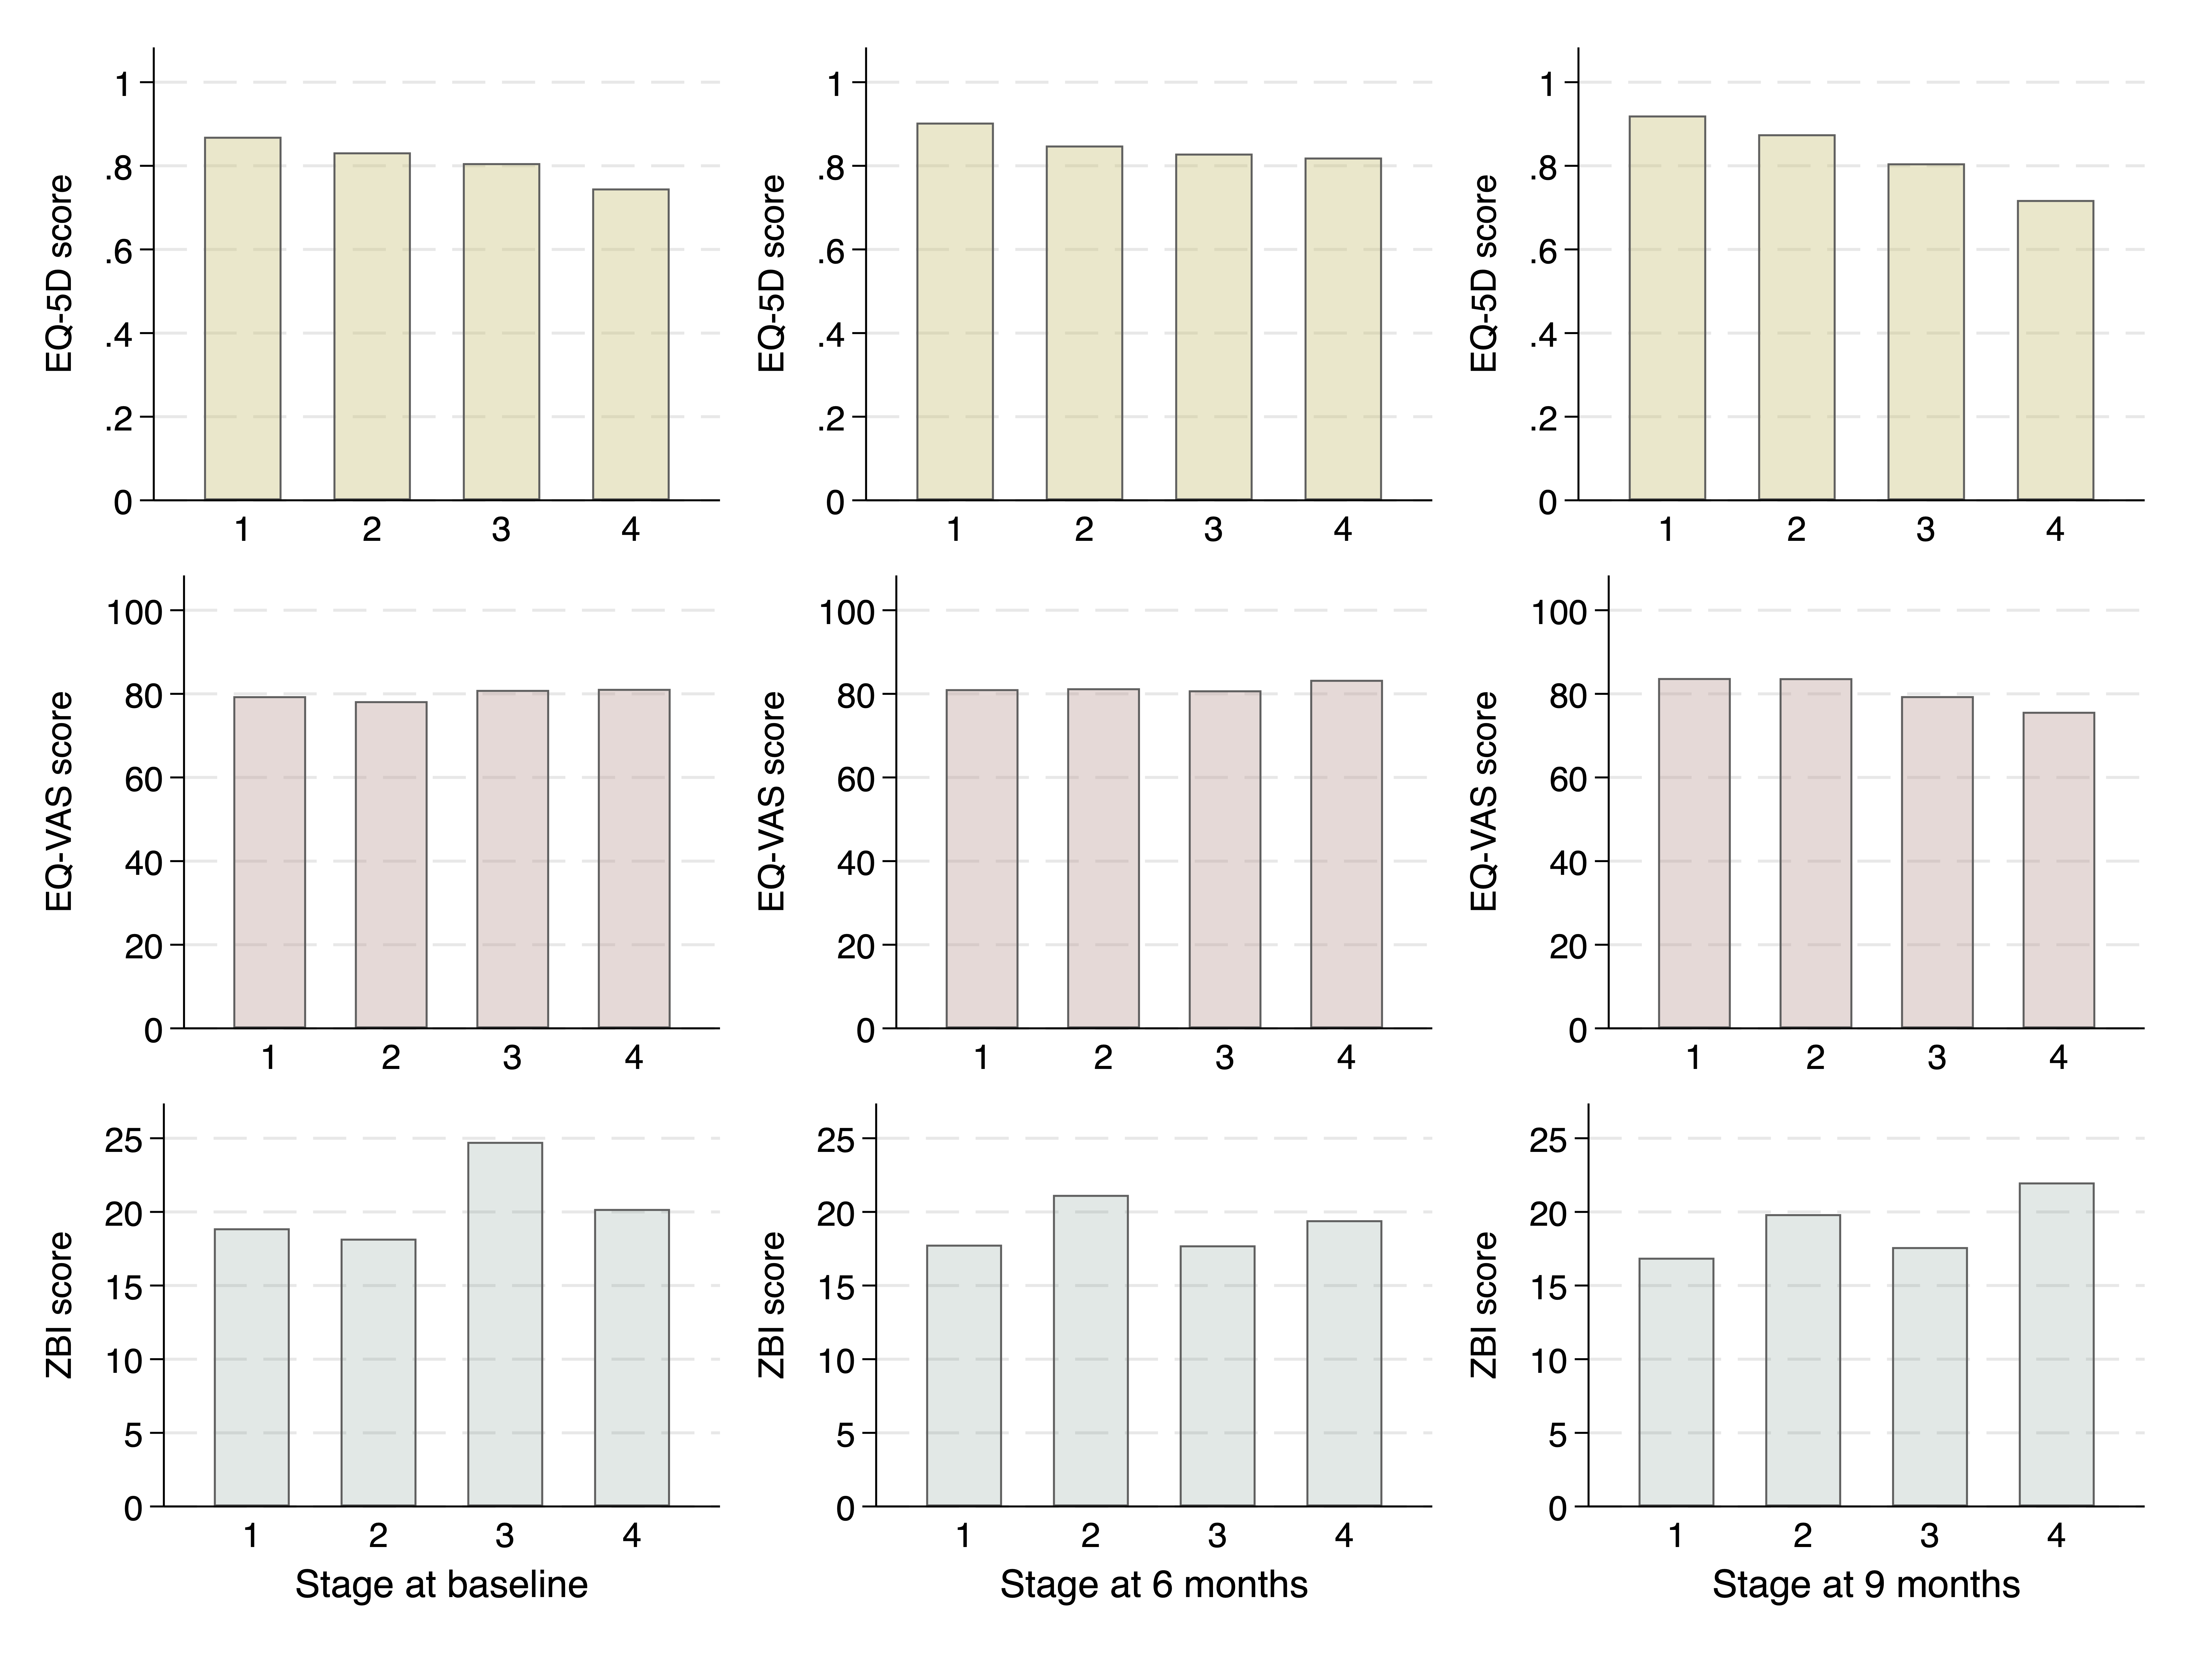
\includegraphics[width=1\linewidth]{figures/outcome-kings-stage.png}
    \caption{EQ-5D-5L utility scores, domain scores and scores by King’s stage}
    \label{fig:outcome-kings-stage}
    \caption*{\footnotesize \textit{Notes:} ANOVA, analysis of variance; EQ-5D, EuroQol 5-dimension questionnaire; VAS, visual analog scale; ZBI, Zarit Burden Interview}
\end{figure}

\begin{table}[H]
    \centering \singlespacing \small
    \caption{Pooled carer ZBI, EQ-VAS, and EQ-5D utility and domain scores by King’s stage}
    \begin{tabular}{|L{.33\linewidth}|R{.1\linewidth}|R{.1\linewidth}|R{.1\linewidth}|R{.1\linewidth}|R{.1\linewidth}|}
        \hline
        \PlainInput{tables/tab_outcomes_kings}
    \end{tabular}
    \label{tab_outcomes_kings}
    \caption*{\footnotesize 
                \textit{Notes:} Data from all caregivers at all time points (baseline, 6 months, and 9 months) have been pooled. Comparisons of outcomes between King’s stages use ANOVA. ZBI total score ranges from 0 to 88, with higher scores indicating greater burden. EQ-5D scores range from 0 to 1.0, with higher scores indicating better health-related quality of life. EQ-VAS scores range from 0 to 100, with higher scores indicate better health-related quality of life. EQ-5D domain scores range from 0 to 3, with higher scores indicating greater restriction by domain. \\
                ANOVA, analysis of variance; EQ-5D, EuroQol 5-dimension questionnaire; VAS, visual analog scale; ZBI, Zarit Burden Interview}
\end{table}

\subsection*{Caregiver HRQoL and burden over time}
\autoref{tab_outcomes_time} The mean (SD) change in carers ZBI scores from baseline to 18 months was X.X (X.X) for the caregiver EQ-5D index score,X.X (X.X) for the caregiver EQ-5D VAS score, and X.X (X.X) for the ZBI score. For the two HRQoL measures, the change from baseline to 6 months or 9 months was not significant. We found significant differences in ZBI scores between 0 and 9  months (p value = X.XXX), mostly driven by the change ins cores beuween 0 and 6 months. 

\autoref{fig:eq5d-domains-time} shows the EQ-5D domain scores over time. At baseline, no caregiver had any problem in self-care domain. %Examination of the EQ-5D domain scores (Fig. 1) showed that very few caregivers had extreme problems (<5\% for any domain) and the levels of problems were similar at baseline and at 18 months. At both time points, more caregivers had some problems in the domains of pain/discomfort (baseline: 42.8\%; 18 months: 46.8\%) and anxiety/depression (baseline: 30.3\%; 18 months: 33.9\%) than in the other three domains.

\begin{table}[H]
    \centering \singlespacing \small
    \caption{Means differences (95\% confidence intervals) and p-values from t-tests comparing of caregiver ZBI, EQ-VAS, and EQ-5D scores changes over time}
    \begin{tabular}{|L{6cm}|C{5cm}|C{2.5cm}|}
        \hline
        \PlainInput{tables/tab_outcomes_time}
    \end{tabular}
    \label{tab_outcomes_time}
    \caption*{\footnotesize 
                \textit{Notes:} CI, confidence interval; EQ-5D, EuroQol 5-dimension questionnaire; VAS, visual analog scale; ZBI, Zarit Burden Interview}
\end{table}

\begin{figure}[H]
    \centering
    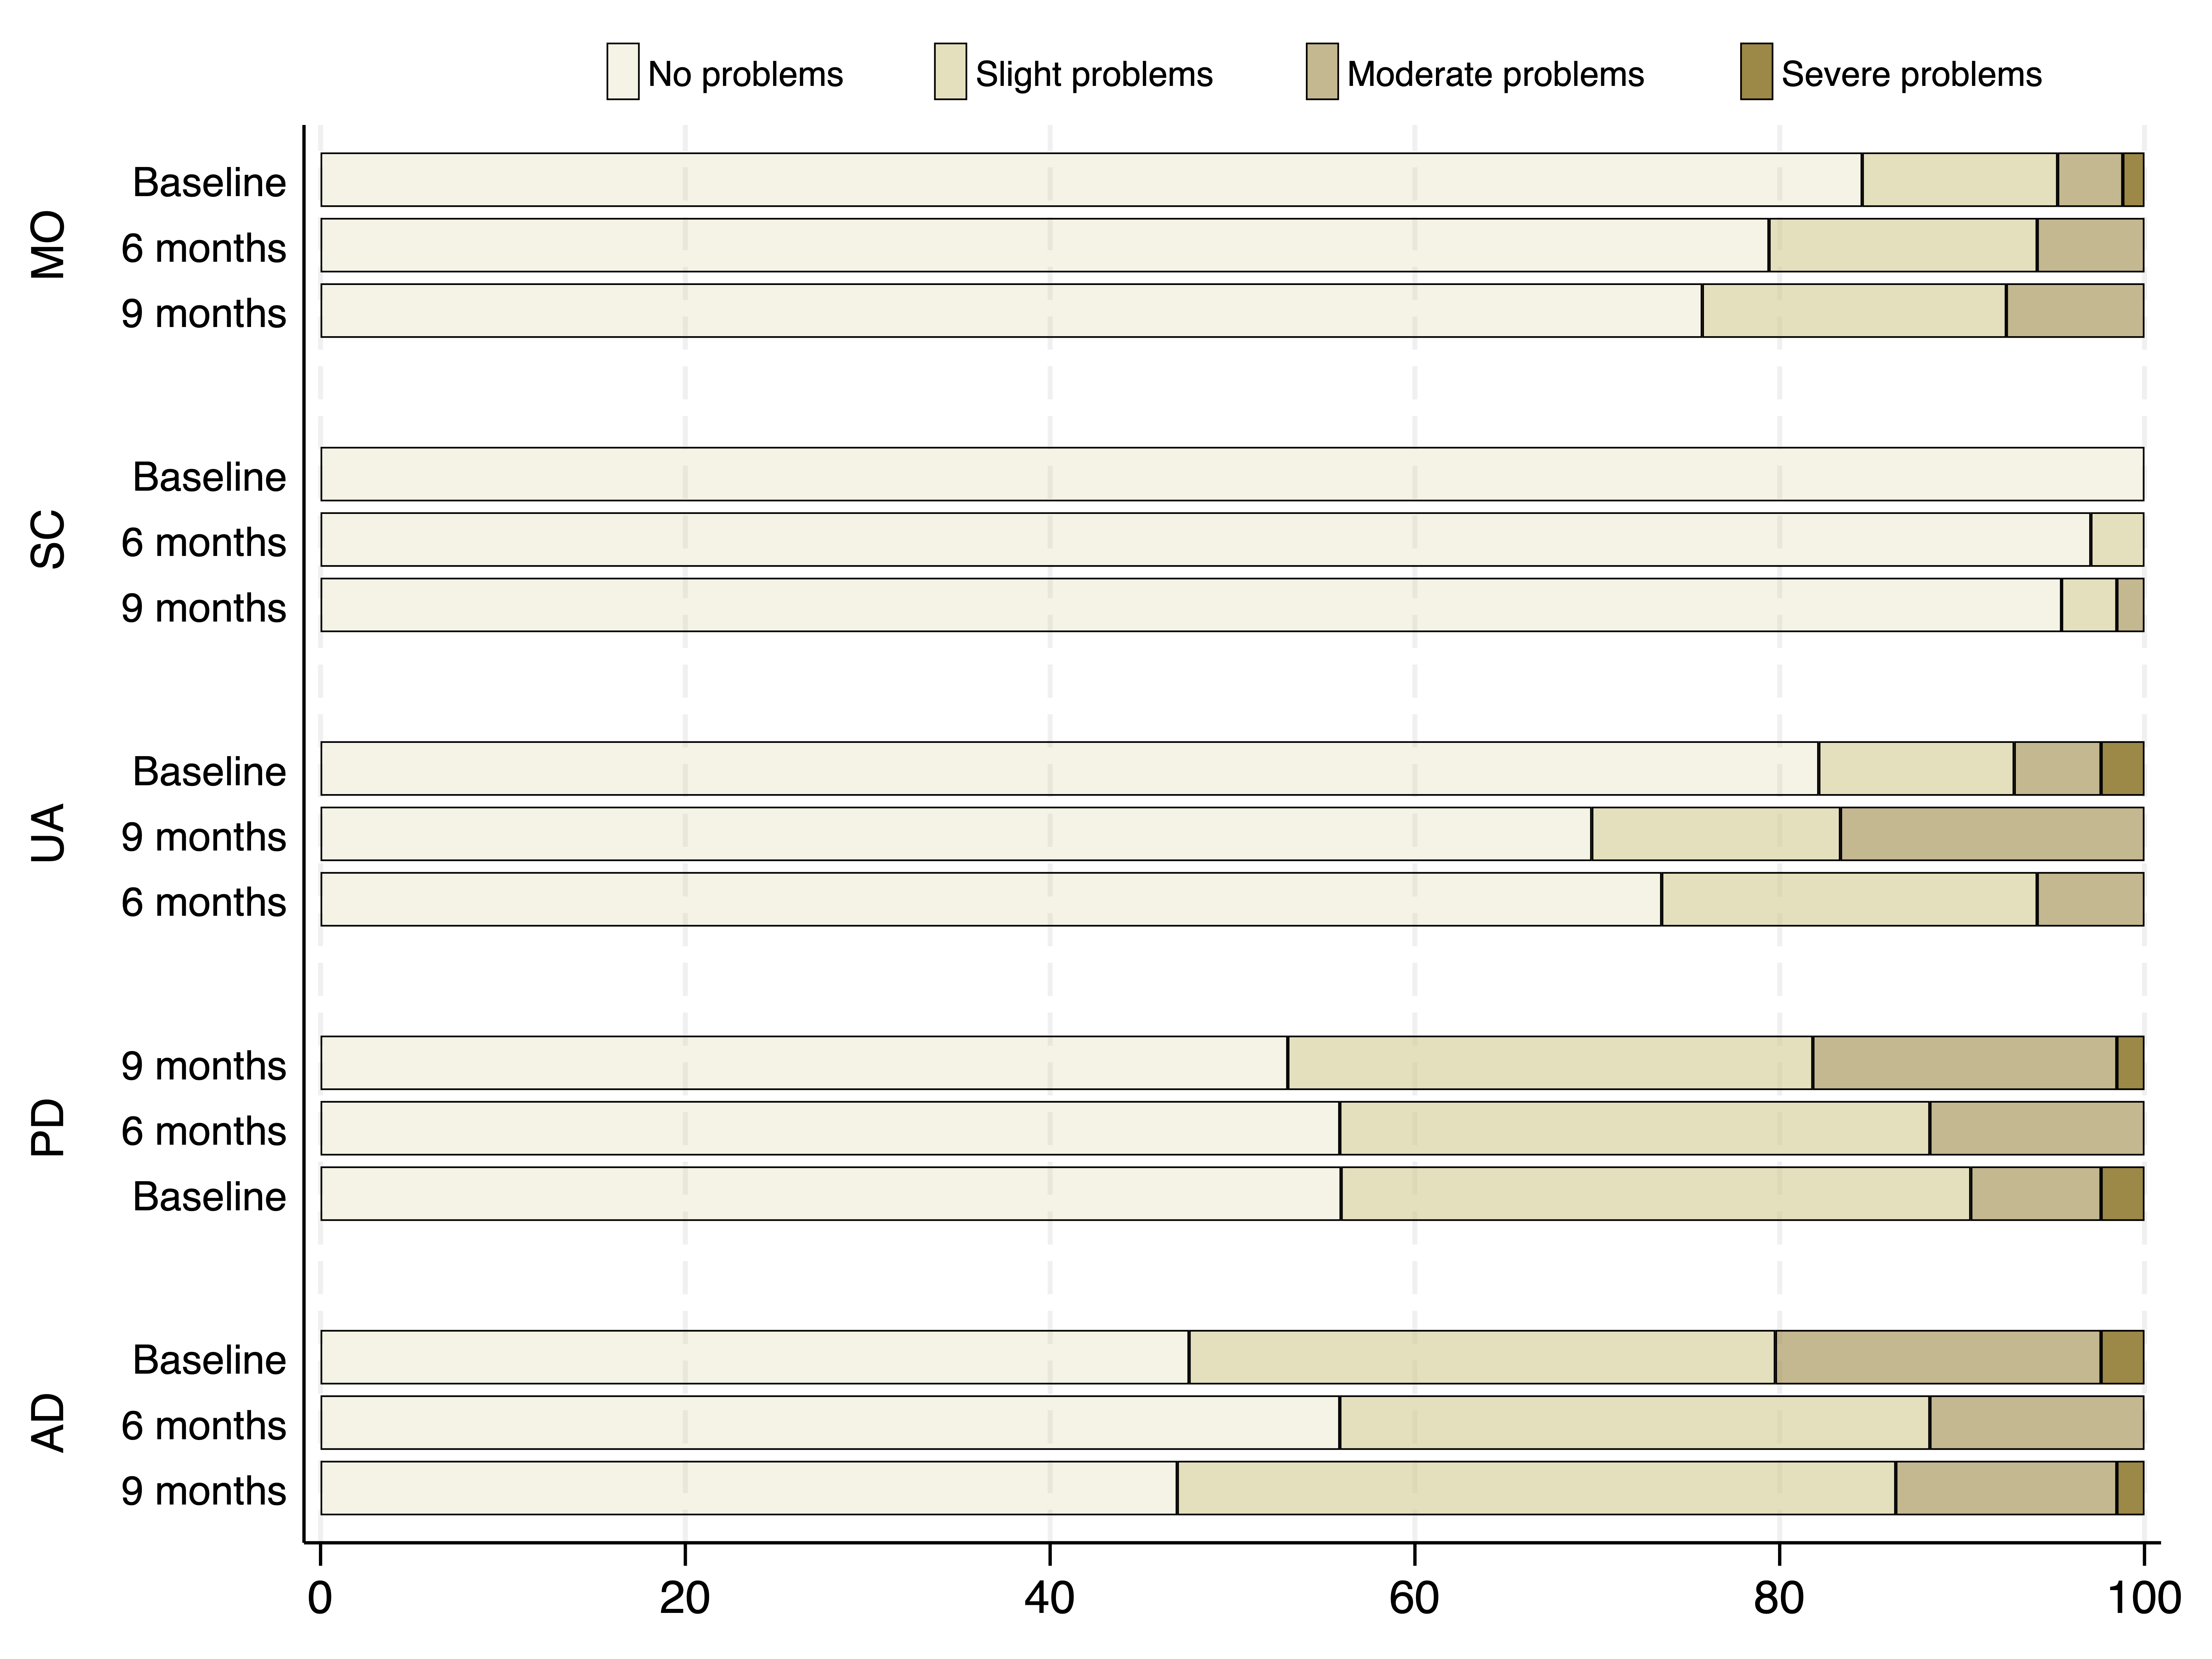
\includegraphics[width=1\linewidth]{figures/eq5d-domains-time.png}
    \caption{Problems in the caregiver EQ-5D domains at baseline, 6 months, and 9 months.}
    \label{fig:eq5d-domains-time}
    \caption*{\footnotesize \textit{Notes:} MO, mobility; SC, self-care; UA, usual activities; PD, pain/depression; AD, anxiety/depression.}
\end{figure}

\subsection*{Relationship between ZBI and EQ-5D}
Correlations were weak or very weak between EQ-5D (index and VAS scores) and ZBI at each time point and for the change scores (\autoref{tab_outcomes_corr}). For the ZBI, the 18-month change score correlation was −0.16 (95\% confidence interval, CI: −0.22, −0.09) for the EQ-5D VAS score and −0.09 (95\% CI: −0.15, −0.03) for the EQ- 5D index score.

\begin{table}[H]
    \centering \singlespacing \small
    \caption{Spearman correlation coefficients between caregiver burden and quality of life scores at baseline, at 9 months, and change in scores between baseline and 9 months.}
    \begin{tabular}{|L{3.6cm}|C{1.7cm}|C{1.4cm}|C{1.7cm}|C{1.4cm}|C{1.7cm}|C{1.4cm}|}
        \hline
        \PlainInput{tables/tab_outcomes_corr}
    \end{tabular}
    \label{tab_outcomes_corr}
    \caption*{\footnotesize 
                \textit{Notes:} EQ-5D, EuroQol 5-dimension; EQ-VAS, EuroQol visual analog scale; ZBI, Zarit Burden Interview}
\end{table}

\subsection*{Factors influencing caregiver burden}
%As already shown above, the patient’s functional status had a clear influence on her/his caregiver’s burden. To provide a deeper analysis of further influencing factors on caregiver burden (ZBI score), multiple regression analysis was used (Table 3). The patient’s wheelchair dependency increased the ZBI score by 9.30 points. Additionally, a rise of 5.01 points was observed, if the patient needed permanent supervision. The main influence on the ZBI appeared to be the CG’s mental health impairment due to caregiving with an increase of 11.36 points. However, physical health impairment had no statistically significant impact on the ZBI score. Furthermore, patients’ age seemed to slightly lower the burden by −0.24 points for each increasing year. Neither the patient’s nor the CG’s gender had statistically significant impacts on the ZBI in the multivariate regression analysis.

\begin{table}[H]
    \centering \singlespacing \small
    \caption{Multivariable OLS regression models of associations between caregiver burden (ZBI) and caregiver- and patient-related independent variables}
    \begin{tabular}{|L{5cm}|R{1.6cm}|R{1.6cm}|R{1.6cm}|R{1.6cm}|R{1.6cm}|}
        \hline
        \PlainInput{tables/tab_multiOLS_zbi}
    \end{tabular}
    \label{tab_multiOLS_zbi}
    \caption*{\footnotesize 
                \textit{Notes:} ALSFRS-R, Revised Amyotrophic Lateral Sclerosis Functional Rating Scale; MQOL, McGill Quality of Life Questionnaire; ZBI, Zarit Burden Interview}
\end{table}



\begin{table}[H]
    \centering \singlespacing \small
    \caption{Multivariable OLS regression models of associations between health‐related quality of life (EQ-5D) and caregiver- and patient-related independent variables}
    \begin{tabular}{|L{5cm}|R{1.6cm}|R{1.6cm}|R{1.6cm}|R{1.6cm}|R{1.6cm}|}
        \hline
        \PlainInput{tables/tab_multiOLS_eq5d}
    \end{tabular}
    \label{tab_multiOLS_eq5d}
    \caption*{\footnotesize 
                \textit{Notes:} ALSFRS-R, Revised Amyotrophic Lateral Sclerosis Functional Rating Scale; EQ-5D, EuroQol 5-dimension; MQOL, McGill Quality of Life Questionnaire}
\end{table}


\clearpage
\section*{Supplementary tables}


\begin{table}[H]
    \centering \singlespacing \small
    \caption{Multivariable Beta regression models of associations between caregiver burden (ZBI) and caregiver- and patient-related independent variables}
    \begin{tabular}{|L{5cm}|R{1.6cm}|R{1.6cm}|R{1.6cm}|R{1.6cm}|R{1.6cm}|}
        \hline
        \PlainInput{tables/tab_multiBeta_zbi}
    \end{tabular}
    \label{tab_multiBeta_zbi}
    \caption*{\footnotesize 
                \textit{Notes:} ALSFRS-R, Revised Amyotrophic Lateral Sclerosis Functional Rating Scale; MQOL, McGill Quality of Life Questionnaire; ZBI, Zarit Burden Interview}
\end{table}



\begin{table}[H]
    \centering \singlespacing \small
    \caption{Univariable OLS regression models of associations, with ZBI as dependent variable, used in selection of independent variables for multivariable regression}
    \begin{tabular}{|L{6cm}|C{2cm}|C{3cm}|C{2cm}|}
        \hline
        \PlainInput{tables/tab_univarReg_zbi}
    \end{tabular}
    \label{tab_univarReg_zbi}
    \caption*{\footnotesize 
                \textit{Notes:} ALSFRS-R, Revised Amyotrophic Lateral Sclerosis Functional Rating Scale; HADS, Hospital Anxiety and Depression Scale; MQOL, McGill Quality of Life Questionnaire; ZBI, Zarit Burden Interview}
\end{table}



\begin{table}[H]
    \centering \singlespacing \small
    \caption{Univariable OLS regression models of associations, with EQ-5D as dependent variable, used in selection of independent variables for multivariable regression}
    \begin{tabular}{|L{6cm}|C{2cm}|C{3cm}|C{2cm}|}
        \hline
        \PlainInput{tables/tab_univarReg_eq5d}
    \end{tabular}
    \label{tab_univarReg_eq5d}
    \caption*{\footnotesize 
                \textit{Notes:} ALSFRS-R, Revised Amyotrophic Lateral Sclerosis Functional Rating Scale; HADS, Hospital Anxiety and Depression Scale; MQOL, McGill Quality of Life Questionnaire; ZBI, Zarit Burden Interview}
\end{table}



%%%%%%%%%%%%%%%%%%%%%%%%%%%%
%%% %%%
%%% Bibliography %%%

\clearpage
\newrefcontext[sorting=nyt]
\printbibliography


\end{document}